\section{Diskussion}

Das kleinere, ausschließlich mit literaturbasierten Features trainierte Modell erreichte mit 87\% bereits eine relativ hohe Präzision.
Dies kann dahingehend interpretiert werden, dass die genutzten Features grundsätzlich geeignet sind um verschöwrungstheoretische Texte von anderen zu Unterscheiden.
Die verwendete \textit{lightGBM} Software erlaubt es die Bedeutung einzelner Features für das erstellte Modell abzuschätzten.
Das Features mit dem höchsten Informationszuwachs (Gain) für das Modell ist die Anzahl der internen Links (Gain = $0.12$).
Die Anzahl der externen Links hingegen bot einen deutlich geringeren Gain ($0.076$) für das Modell.
Dies ist insofern bemerkenswert, als dass die in der Literatur gemachten Beobachtungen wie etwa die von \textcite[10]{soukup_2008} hätten vermuten lassen, dass die Verknüfung mit externen Quellen ein wichtigeres Merkmal ist als die mit internen.

Die nächstwichtigen Features sind die Anzahl der eingebundenen Bilder (Gain = $0.1$), die Summe der Sentimente ($0.1$) und der Anteil an zitierten Text ($0.9$).
Interessant ist hier noch, dass anders als die Summe an Sentimentscores der Betrag der Sentimentscores für die Klassifizierung relativ unbedeutend ist (Gain = $0.018$).
Dies kann zum einen daran liegen, dass diese Werte nicht vollständig unabhängig voneinander sind und der Trainingsalgorithmus deshalb u.U. nur einen der Werte berücksichtigt.
Zum anderen kann es aber auch ein Indiz sein, dass Verschwörungstheoretische Texte nicht notwendigerweise allgemein emotionaler sind, aber im Schnitt deutlich negativere Sentimente Transportieren wie sich auch an den Durchschnittswerten der Sentimentsumme zeigt ($\overline{X} = -4.22$ gegenüber $\overline{X} = -1.35$).

Die meisten anderen Features lieferten dem Modell einen mittelgroßen Informationszuwachs, besonders wenig nützlich waren vor allem Features die mehr oder weniger mit anderen Features zusammenhängen (die Summe positiver bzw. negativer Sentimente, Zahl der direkten Zitate, etc.), die Menge an Negationen, an Zahlenangaben sowie allgemein an eingebetteten Medien (Twitter, Youtube, Sonstige).
Eine Erklärung für letztere könnte dabei aber auch schlicht sein, dass herkömmliche Medien inzwischen solche Medien auch häufiger einbinden und in diesem stilistischen Merkmal sich den Verschwörungstheorien angenähert haben.

Es bleibt anzumerken, dass Verfahren des Maschinellen Lernenes, wie hier Gradientenboosting, komplexe Systeme sind und selbst wenn wie hier der Einfluss einzelner Features auf das Modell abgeschätzt werden kann, die Interpretation solcher Ergebnisse immer schwierig und zu einem gewissen Teil spekulativ ist.

\begin{figure}[h]
    \centering
    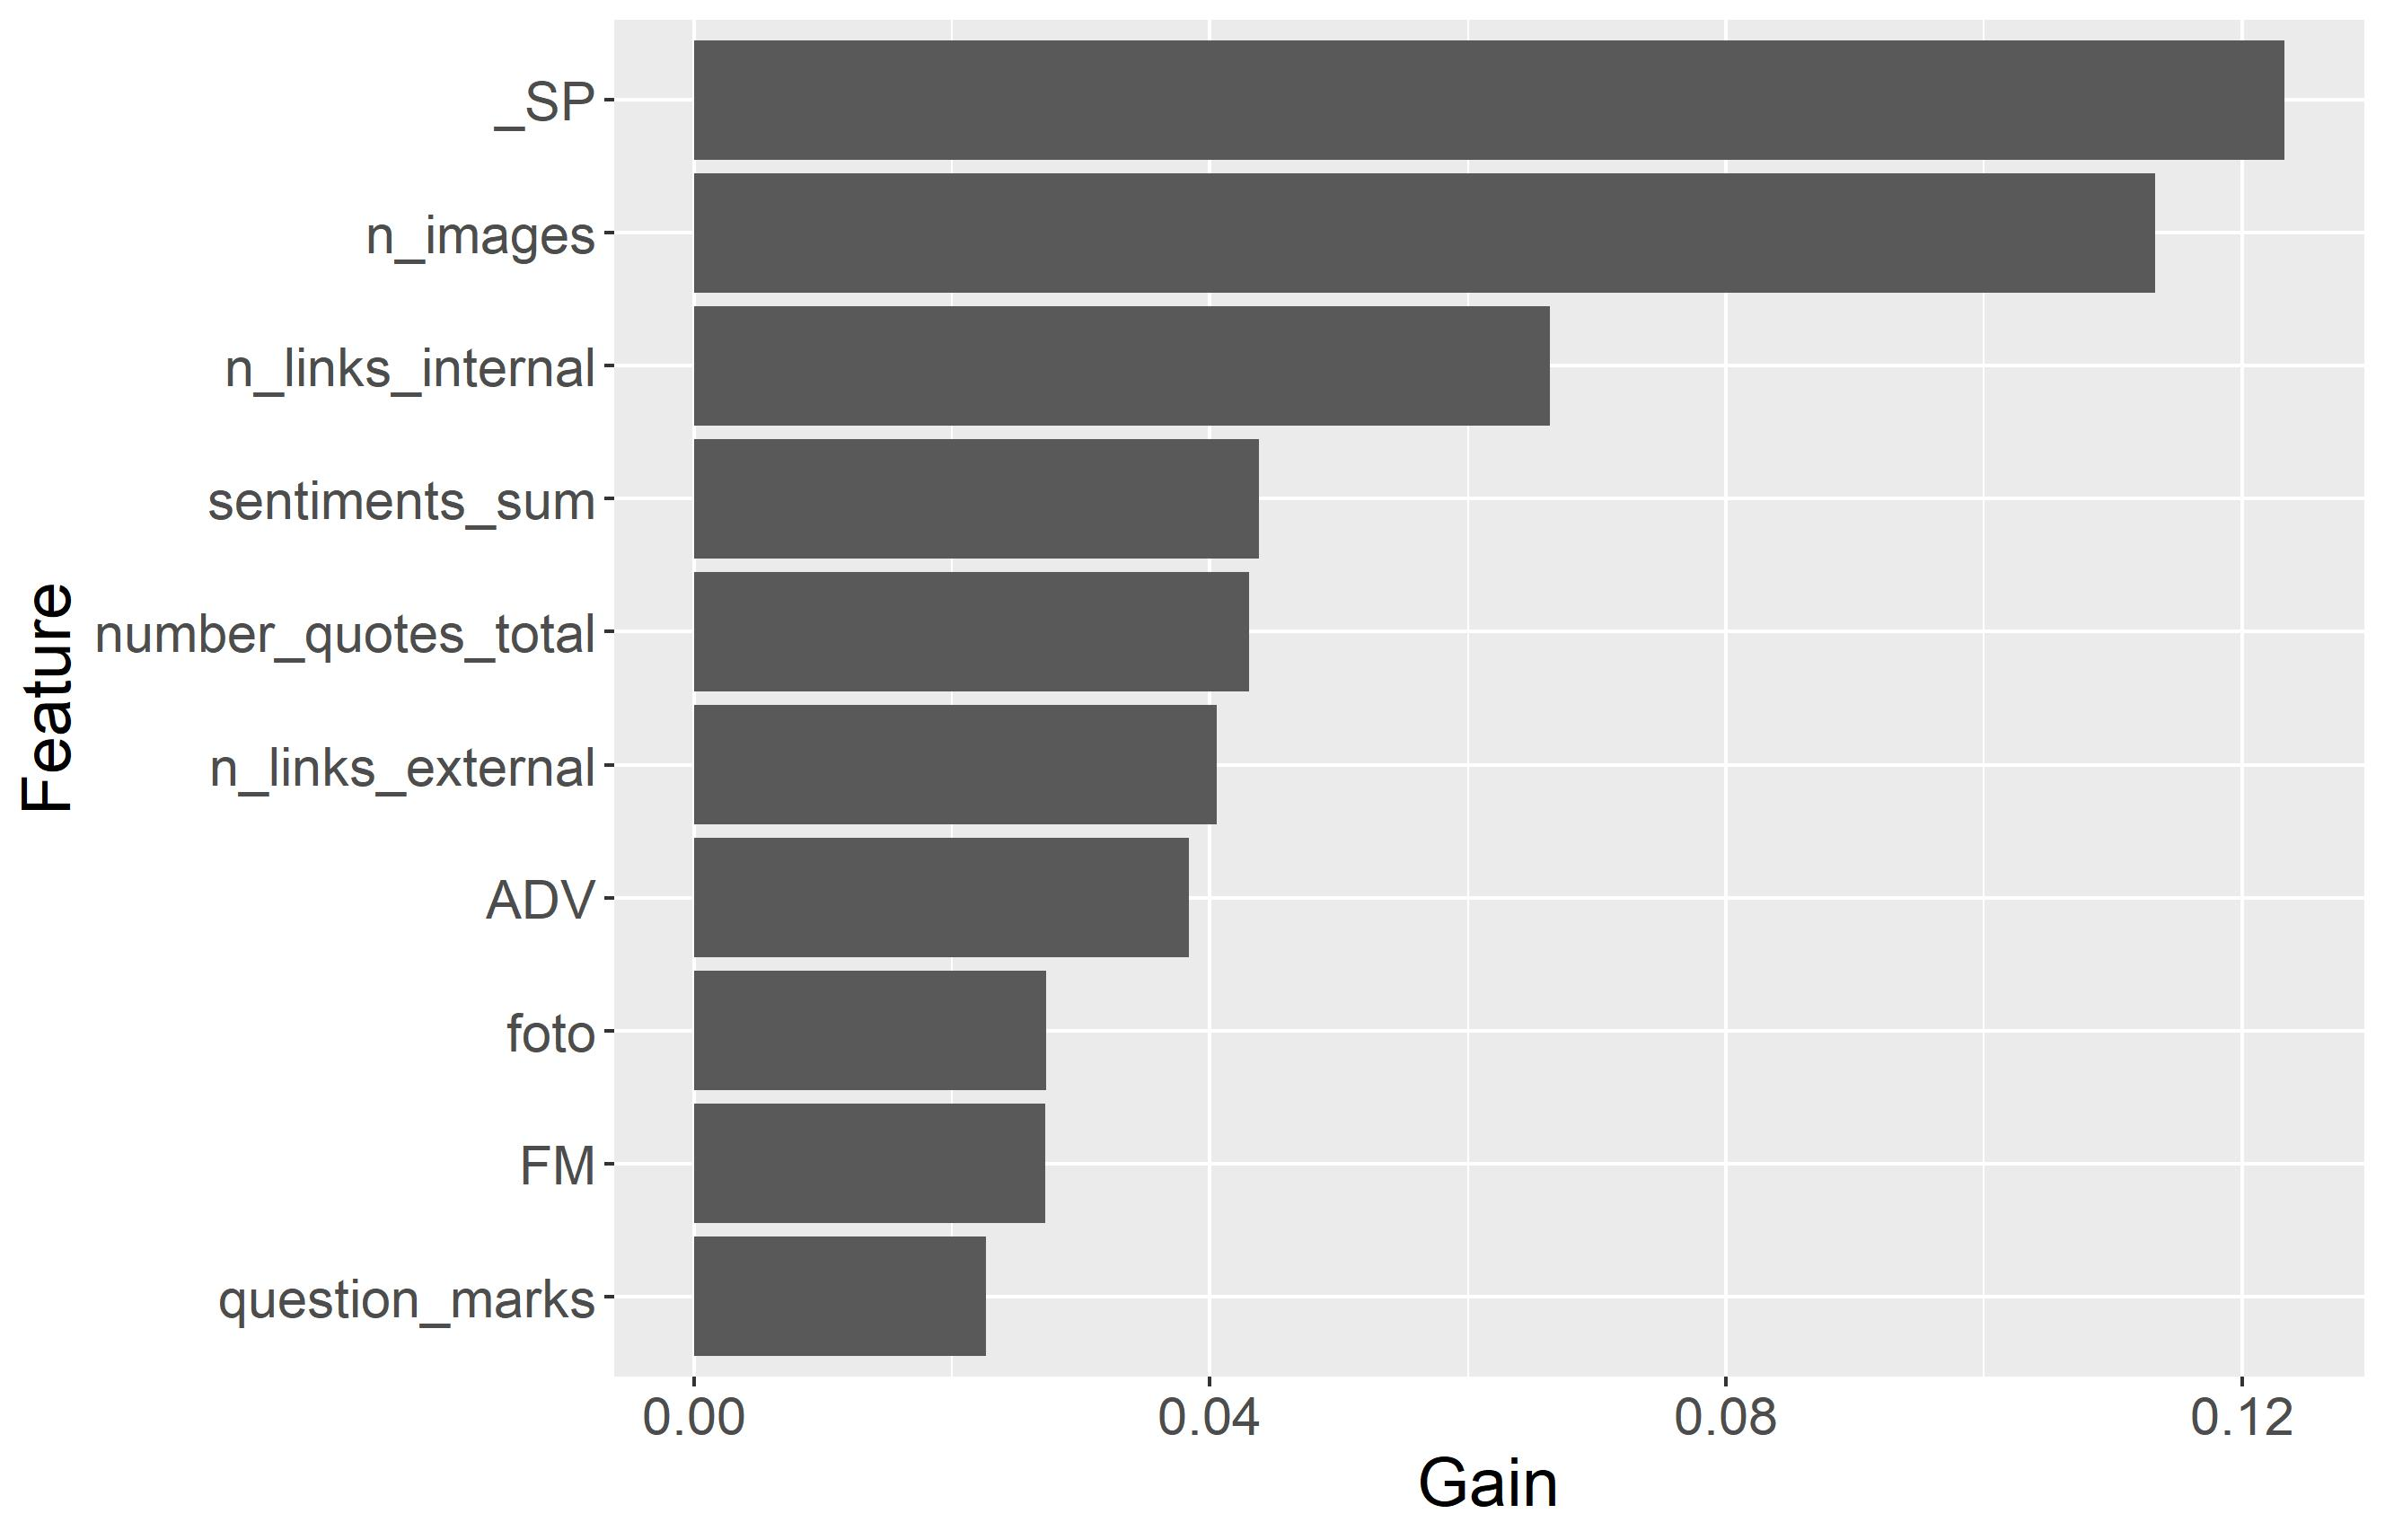
\includegraphics[scale=0.45]{graphics/top_10_features.jpg}
    \caption{Top-10 Features nach Bedeutung für das Modell. Namen in Großbuchstaben = Part-of-Speech Tag; Namen in kleinbuchstaben = tf-idf Worthäufigkeit; Benannte Features = Auf Literatur basierende Statistiken}
    \label{top-features}
\end{figure}

\FloatBarrier

Das vollständige Modell erreichte mit fast 98\% eine sehr gute Präzision.
Es kann zuverlässig zwischen den Verschwörungstheoretischen Texten und dem Vergleichskorpus unterscheiden.
Eine Betrachtung der wichtigsten Features aus Grafik \ref{top-features} zeigt zunächst, dass viele der auch im ersten Model wichtigen Features wieder von großer Bedeutung sind (Zahl der Bilder, Zahl der internen Links, Summe der Sentimentscores und Anteil von zitiertem Text).
Einige der Wortfrequenzen mit dem meisten Einfluss auf die Klassifizierungen sind foto, krieg, merkel und regierung.
Die meisten davon sind durchaus erwartbare Ergebnisse, die Verwendung von Worten aus solchen Themenbereichen ist in der Literatur gut belegt, etwa bei \textcite[150]{stumpf_2019} oder \textcite[25]{uscinski_2014}.
Unter den wichtigen POS Tags sind Leerzeichen, Adverben, für fremdsprachigen Text (meist englischer Text, häufig zitiert) und für Coordinating Conjunctions (also Wörtern wie und, oder, aber, etc.\parencite*[vgl.][]{smith_2003}).
Interessant ist auch, dass die Zahl der Fragezeichen im kleineren Modell zwar kaum relevant ist, im größeren Modell aber unter den 10 einflussreichsten Features.

Eine mögliche Erklärung für die überraschend gute Leistung des trainierten Modells ist, dass die relativ geringe Vielfalt insbesondere des Ausgangskorpuses einen Teil zu der guten Leistung beigetragen hat.
Auch wenn etwa für \textit{Watergate.tv} mehrere Autor:innen schreiben, ist zu vermuten dass die totale Anzahl an Autor:innen im Korpus im niedrigen zweistelligen Bereich liegt.
Da für die Modellerstellung mit POS-Tags auch eher stilistische Features enthalten sind, ist es durchaus möglich, dass ein Teil der Leistung des Modells weniger auf verschwörungstheoretischen Merkmalen beruht als auf dem Stil der individuellen Autor:innen.

Dieser Faktor dürfte in Kombination mit der relativ geringen Quellenzahl des Korpuses als auch des Vergleichskorpuses die Wahrscheinlichkeit, dass das hier trainierte Modell gut generalisiert deutlich verringern.